
\section{Introduction}

TODO: add citations

Hardware HEVC encoders have recently appeared on consumer-grade GPUs, opening the door to mass 360-degree and 4K video livestreaming. However, traditional methods of adaptive bitrate (ABR) streaming do not work on these ultra-high definition (UHD) videos because they will either be too large for continuous playback or of too low a quality to be enjoyable. A body of work on tile-based ABR streaming for UHD video has recently appeared in which the quality requested for each section of a video corresponds roughly to how interesting it is, allowing end-users to view the most important parts of a video in high-quality without stalling. This is straightforward for pre-rendered videos, but is more complicated in a livestreaming scenario because each quality requires another encode, introducing some delay in the availability of each new segment. Furthermore, tiling is not supported by existing hardware encoders. One can try to get around this by feeding each tile to the encoder as a separate video and stitching them together afterwards, but this requires cropping once for each desired tile in the image on every frame, then swapping out encoder contexts and encoding each tile separately, introducing considerable overhead.

To combat these challenges, we introduce Real-time Adaptive Three-sixty Streaming, or RATS. RATS is a GPU-based HEVC encoding platform to tile, encode, and stitch video at multiple qualities in real-time on a frame-by-frame basis. The source video stream is divided into the desired tile columns and are stacked on top of one another. The rearranged video image is fed to the hardware encoder with slice boundaries specified to at least be the edges of the source video. This process occurs twice for each frame with different bitrate configurations, resulting in high-quality and low-quality outputs. When the video is reconstructed during playback, each tile is an independent region of the frame, allowing us to pick where each tile should appear in the final video and which bitrate it should be.

The rest of this paper is organized as follows: In Section 2, we provide a brief summary of the HEVC encoding process and the NVENC hardware encoder. In Section 3, we describe the proposed system in detail. In Section 4, we sketch out a full web-based video streaming platform centered around RATS. In Section 5, we provide an evaluation of the system. Finally, Section 6 concludes the work.

\renewcommand{\figurename}{Fig.}
\begin{figure*}[t]
	\centering
	\includegraphics[width=0.8\textwidth]{figures/Streaming_scenario_v3.pdf}
	\caption{Adaptive $360\,^{\circ}$ Livestreaming: In this demo we show hardware encoding that allows re-encoding and stitching single tiles of the $360\,^{\circ}$ video in different quality levels (see pipeline). The lower part of the figure shows the demo setup in a streaming infrastructure that makes use of HTTP adaptive streaming.}
\end{figure*}

\section{HEVC and NVENC}

TODO: revise this, add a couple citations

The most computation-heavy components of the HEVC encoding process, such as motion estimation, are not easily parallelized. Parallel HEVC video encoding instead relies on dividing each frame of the video into independent regions, encoding them separately, and joining their edges during playback. Two versions of this concept, slices and tiles, exist within the HEVC standard. Functionally, they are identical; however, slices are limited to chunking the video into wide strips, while tiles can divide a video into rectangular CTU-based areas of any size. While tiles are supported by most decoders, very few encoders allow for it, all of which are software encoders far too slow to operate in real-time.

HEVC encoders convert raw video into an HEVC bitstream consisting of multiple sequential NAL units via a complex implicit syntax. Each NAL unit contains some header information followed by raw image data. For videos without slicing or tiling, most NAL units correspond to a single full frame of video; however, because slices and tiles are independently-decodable, each tile or slice within a video frame is a self-contained NAL unit. Interestingly, we can then treat any rectangular arrangement of HEVC bitstreams as tiles within a single video by alternating their NAL units and manipulating specific values in the NAL headers. This process, in which multiple bitstreams are joined to form one bitstream which displays all constituent bitstreams in different regions of the final video, is known as \textit{stitching}. (Maybe include some references to works which do stitching or something)

NVENC is a hardware video encoder present on newer Nvidia GPUs, and is the state-of-the-art hardware HEVC encoder. Note that HEVC is not easily data-parallelizable; as a result, NVENC is an ASIC separate from the CUDA cores. Interaction with NVENC occurs via the NVENCODE API, and offers the user a handful of parameters for the encoder, such as target bitrate, slice boundaries, and GOP specifications. It is possible to swap out encoder configurations between frames, allowing one to encode multiple videos simultaneously, but even top-of-the-line consumer GPUs only support a maximum of two contiguous configurations by default. Note that these configurations are not simply encoding parameters, but also contain the previous frame data necessary to encode the next P- or B-frame. These configurations must therefore exist continuously throughout the encoding process. This is a limitation enforced by the driver, and supercomputing GPUs, such as the Nvidia Titan V, do not have such limits. Such GPUs are prohibitively expensive for most consumers, so we do not consider them here.

\section{RATS Implementation}
To work within the confines imposed by NVENC, namely the lack of tile support and limitation to two simultaneous encoding sessions, we divide the real-time adaptive encoding pipeline into an encoding component, in which a raw video frame is manipulated and converted into low- and high-quality bitstreams, and a stitching component, in which these bitstreams are combined to be displayed to the user.

\subsection{Encoding}

TODO: revise

NVENC supports multiple slice modes, one of which, \texttt{sliceMode=3}, cuts the video into $n$ equal slices as specified via the \texttt{sliceModeData=}$n$ parameter. Vertical cuts, which are important for 360-degree video, cannot be made via slices, but the image boundaries are natural slice boundaries as well. We therefore manipulate the input images by vertically cutting them into $n$ pieces of equal size and stacking these pieces on top of each other, then setting \texttt{sliceModeData=}$n$, so that the slice boundaries align with the top and bottom boundaries of the original image. To ensure the stacked image is divided evenly, the CTU height of the image must be divisible by the desired number of tile rows. Similarly, the width of the image must be divisible by the number of tile columns to keep stacked columns the same width. We thus crop the input video if necessary, but one could also resize the input video or simply reject it. The output bitstream from the encoder will typically contain $n+1$ NAL units per frame, one for each slice and a single SEI at the end. During the stitching process, specific changes will be made to the NAL headers to instead treat these slices as tiles and place them side-by-side in the final video bistream.

In a YUV420p video, each frame of the video consists of the titular Y, U, and V components, corresponding to the luminance and two chrominance components, respectively. These components are laid out sequentially as well, such that the luminance of the image is described, then one chrominance component, then the other. Each byte within the luminance component corresponds to a single pixel in the image, but each byte within a chrominance component corresponds to a $2\times2$ pixel area. Either chrominance component is therefore a quarter of the size of the luminance component.

Rearranging is performed on each component via memcpy, with a length equal to the width of a tile column. Recall that the purpose of rearranging is to set the vertical tile boundaries, as NVENC slicing will handle the horizontal tile boundaries. Within each tile column, we begin at the first pixel row and move down, calling memcpy on each pixel row and placing the contents in a new array, before moving on to the next tile column once we hit the bottom of the image. The result of this process will be an image in which the tile columns are effectively stacked on top of one another.

To interact with NVENC, we use the libavcodec API provided by FFmpeg. The high- and low-bitrate configurations are distinct instances of the AVCodecContext struct, which are initialized before the encoding process begins. During the encoding process, a rearranged image is passed to NVENC twice, once with each AVCodecContext instance, to obtain the low- and high-bitrate bitstreams. Within NVENC, we set sliceModeData equal to the total number of tiles desired. The left and right tile boundaries will be the edges of the image fed to NVENC, so the slicing will create the top and bottom boundaries.

\subsection{Stitching}

TODO: revise

The bitstreams resulting from the encoding process contain the independently-decodable slices which will function as our tiles, but they will still be stacked from top-to-bottom. Fortunately, we must only modify a few fields in the NAL headers to convert the slices to tiles and arrange them in the desired configuration. Table ~\ref{tab:stitch} lists all such fields. Note that within an HEVC bitstream, \textit{NAL} and \textit{slice} are equivalent terms which may be used interchangeably. To avoid confusion, we will retain the use of "slice" to refer to an independently-decodable horizontal strip of an image.

In addition to modifying those values listed in Table ~\ref{tab:stitch}, there are two more changes necessary on behalf of emulation prevention bytes and byte alignment. NAL borders are represented by the byte-aligned sequence \texttt{0x000001}. To prevent this sequence from occurring by chance within a NAL, the byte-aligned sequence \texttt{0x03}, referred to as the emulation prevention byte, may be inserted after any \texttt{0x0000} which is not part of a NAL border. The emulation prevention byte has no other meaning and does not otherwise impact the NAL parsing process.

If the stitching process modifies the number of bits in the NAL header by, e.g., inserting a new field or changing the value of an unsigned Exponential Golomb code, any emulation prevention bytes appearing after the point of change will likely cease to be byte-aligned. The decoder will then consider these bits to have semantic value, resulting in a corrupt or incorrect header. We must also ensure that the stitching process does not introduce any new \texttt{0x0000} sequences without a trailing emulation prevention byte. To tackle both of these issues at once, we discard any emulation prevention bytes we encounter in the original NAL and check for any \texttt{0x0000} sequences after our changes have been made. No such concern is necessary for the NAL data because this data will be byte-aligned at the end of the header.

Byte alignment occurs at the end of a NAL header or NAL data. After the last semantic bit, a \texttt{1} is appended to the NAL section, followed by as many \texttt{0}s as necessary to complete the byte. As is the case with emulation prevention bytes, if the size of the NAL header changes during modification, we will likely have an incorrect number of trailing \texttt{0}s. To redo the byte alignment, we find the last \texttt{1} in the original NAL and remove it and everything after it, effectively undoing the previous byte alignment. We then perform byte alignment after our modifications have been made.

The stitching process is performed with the Boost C++ dynamic\_bitstream API, which allows one to read bytes into a vector of bits, manipulate these bits, then convert the bit vector into raw bytes. The high- and low-bitrate configurations are identical except for the specified bitrate, and the resulting NAL headers do not change based on, e.g., content, so the output from NVENC is highly predictable. Therefore, navigating to the right spot in the bitstream and making our changes is a straightforward process.

%%\renewcommand{\figurename}{Tab.}
%%\setcounter{figure}{1}
%%\begin{table*}[t]
%%	\centering
%%	\begin{tabular}{llp{3in}r}
%%		\toprule
%%		NAL Type & Field & Description & Fixed value \\
%%		\midrule
%%		\multirow{2}{*}{SPS} & \texttt{pic\_width\_in\_luma\_samples} & Pixel width of the final video. & \\ \cmidrule[0.5pt]{2-4}
%%		& \texttt{pic\_hidth\_in\_luma\_samples} & Pixel height of the final video. & \\
%%		\midrule[1pt]
%%		\multirow{5}{*}[-5em]{PPS} & \texttt{tiles\_enabled\_flag} & Converts slices to tiles and adds several relevant fields to the bitstream syntax. & \texttt{1} \\ \cmidrule[0.5pt]{2-4}
%%		& \texttt{num\_tile\_columns\_minus1} & Number of tile colums minus 1. & \\ \cmidrule[0.5pt]{2-4}
%%		& \texttt{num\_tile\_rows\_minus1} & Number of tile rows minus 1. & \\ \cmidrule[0.5pt]{2-4}
%%		& \texttt{uniform\_spacing\_flag} & Whether tiles are evenly sized. If \texttt{0}, manual tile boundaries must be specified. & \texttt{1} \\ \cmidrule[0.5pt]{2-4}
%%		& \texttt{loop\_filter\_across\_tiles\_enabled\_flag} & Whether in-loop filtering should be performed across tile boundaries. This is optional, and may be desired if there is less of a difference between the high and low bitrates. & \texttt{1} \\
%%		\midrule[1pt]
%%		\multirow{4}{*}[-6em]{\shortstack{I-slice, \\P-slice}} & \texttt{first\_slice\_segment\_in\_pic\_flag} & Should be \texttt{1} in the top-leftmost tile, and \texttt{0} in all other tiles. If \texttt{0}, the slice segment address must be specified. & \\ \cmidrule[0.5pt]{2-4}
%%		& \texttt{slice\_segment\_address} & The address of the top-leftmost CTU in this tile, beginning from 0 at the top-leftmost CTU in the entire image, and incrementing across the image, moving down and continuing at the end of the row.& \\ \cmidrule[0.5pt]{2-4}
%%		& \texttt{slice\_loop\_filter\_across\_slices\_enabled\_flag} & Similar to the loop filter flag in the PPS, but specifically concerned with in-loop filtering across the left and top boundaries of the tile. & \texttt{1} \\ \cmidrule[0.5pt]{2-4}
%%		& \texttt{num\_entry\_point\_offsets} & Used to treat \texttt{emulation\_prevention\_three\_byte} as part of the tile data, which is not desired here. & \texttt{1} \\
%%		\bottomrule
%%	\end{tabular}
%%	\caption{Table containing all NAL header modifications. The "Fixed value" column contains the bit values of hard-coded fields, such as important flags. Missing values indicate that the value may vary depending on the video and parameters used. In this case, all such values would be encoded using unsigned Expontential-Golomb.}
%%	\label{tab:stitch}
%%\end{table*}
%%\renewcommand{\figurename}{Fig.}
%%\setcounter{figure}{2}
\renewcommand{\figurename}{Tab.}
\setcounter{figure}{1}
\begin{table}
	\begin{tabular}{llr}
		\toprule
		NAL Type & Field & Value \\
		\midrule
		\multirow{2}{*}[-.3em]{SPS} & \texttt{pic\_width\_in\_luma\_samples} & \\ \cmidrule[0.5pt]{2-3}
		& \texttt{pic\_height\_in\_luma\_samples} & \\
		\midrule[1pt]
		\multirow{4}{*}[-1em]{PPS} & \texttt{tiles\_enabled\_flag} & \texttt{1} \\ \cmidrule[0.5pt]{2-3}
		& \texttt{num\_tile\_columns\_minus1} & \\ \cmidrule[0.5pt]{2-3}
		& \texttt{num\_tile\_rows\_minus1} & \\ \cmidrule[0.5pt]{2-3}
		& \texttt{uniform\_spacing\_flag} & \texttt{1} \\
		\midrule[1pt]
		\multirow{3}{*}[-1em]{\shortstack{I-slice, \\P-slice}} & \texttt{first\_slice\_segment\_in\_pic\_flag} & \\ \cmidrule[0.5pt]{2-3}
		& \texttt{slice\_segment\_address} & \\ \cmidrule[0.5pt]{2-3}
		\cmidrule[0.5pt]{2-3}
		& \texttt{num\_entry\_point\_offsets} & \texttt{1} \\
		\bottomrule
	\end{tabular}
	\caption{Table containing all NAL header fields requiring modification. Required literal bit values are provided when necessary. Note that \texttt{num\_entry\_point\_offsets} is an Exponential Golomb-coded number, so a literal bit value of \texttt{1} corresponds to a logical value of 0.}
	\label{tab:stitch}
\end{table}
\renewcommand{\figurename}{Fig.}
\setcounter{figure}{1}

\subsection{Hardware Limitations}

TODO: maybe add citation

In this work, we use the NVIDIA GTX 1080 Ti, a state-of-the-art consumer-grade GPU. We chose this GPU because it is powerful, widely available, and inexpensive enough for the general public. As demonstrated in Section 5, this GPU is capable of encoding video streams much faster than our real-time target. There are, however, two limitations placed upon this GPU that we must consider.

First, the maximum input image size is $8192\times8192$ pixels. Most 360-degree videos are only $3840\times2048$ pixels, but recall that we stack tile columns on top of one another before sending the image to the GPU. The maximum limit is therefore reached with only a few tile columns, forcing us to use wide tile columns which may not be granular enough for ABR streaming. To get around this, we divide the image into multiple sub-images whose columns do not exceed $8192$ pixels when stacked, and encode each of these sub-images independently, once at either bitrate. Specifying more tile columns will thus require additional encodes for each frame, but, fortunately, the GPU encoder is fast enough to keep the total encode time well below the real-time target for realistic tile configurations.

We must make a few small changes to the stitching process to handle sub-images. Note that the location of each tile within a sub-image may not correspond to its location in the final stitched image. For example, consider a video with 6 tile columns. From left to right, let us say the first 4 columns constitute one sub-image, and the final 2 columns constitute another. In this case, the CTU offsets of the first tile row in the first sub-image will remain the same, but the offsets of all other tiles will change in the final image. Because the final image size is different from the size of either sub-image, the number of bits used to encode the CTU offset will change as well. Furthermore, the first tile in the second sub-image will not contain a CTU offset in the NAL header, requiring this field to be inserted at the correct location. Finally, multiple similar parameter sets will be produced, so we keep one and discard the others. Choosing which one to keep is arbitrary, as differing important fields will be modified during the stitching process.

Second, as detailed in Section 2, the GPU driver does not allow more than 2 simultaneous context configurations during the encoding process. Each sub-image at either bitrate requires an independent context configuration, i.e. an instance of AVCodecContext. Each sub-image at either quality requires its own context, so this limitation would normally prevent us from making use of the sub-image technique detailed above. Fortunately, it is possible to remove the 2 context limit by sending a particular bytestream to the GPU. A script to do so is provided in nvidia-patch [CITE, or footnote], which we used for this work.

\begin{figure}[t]
	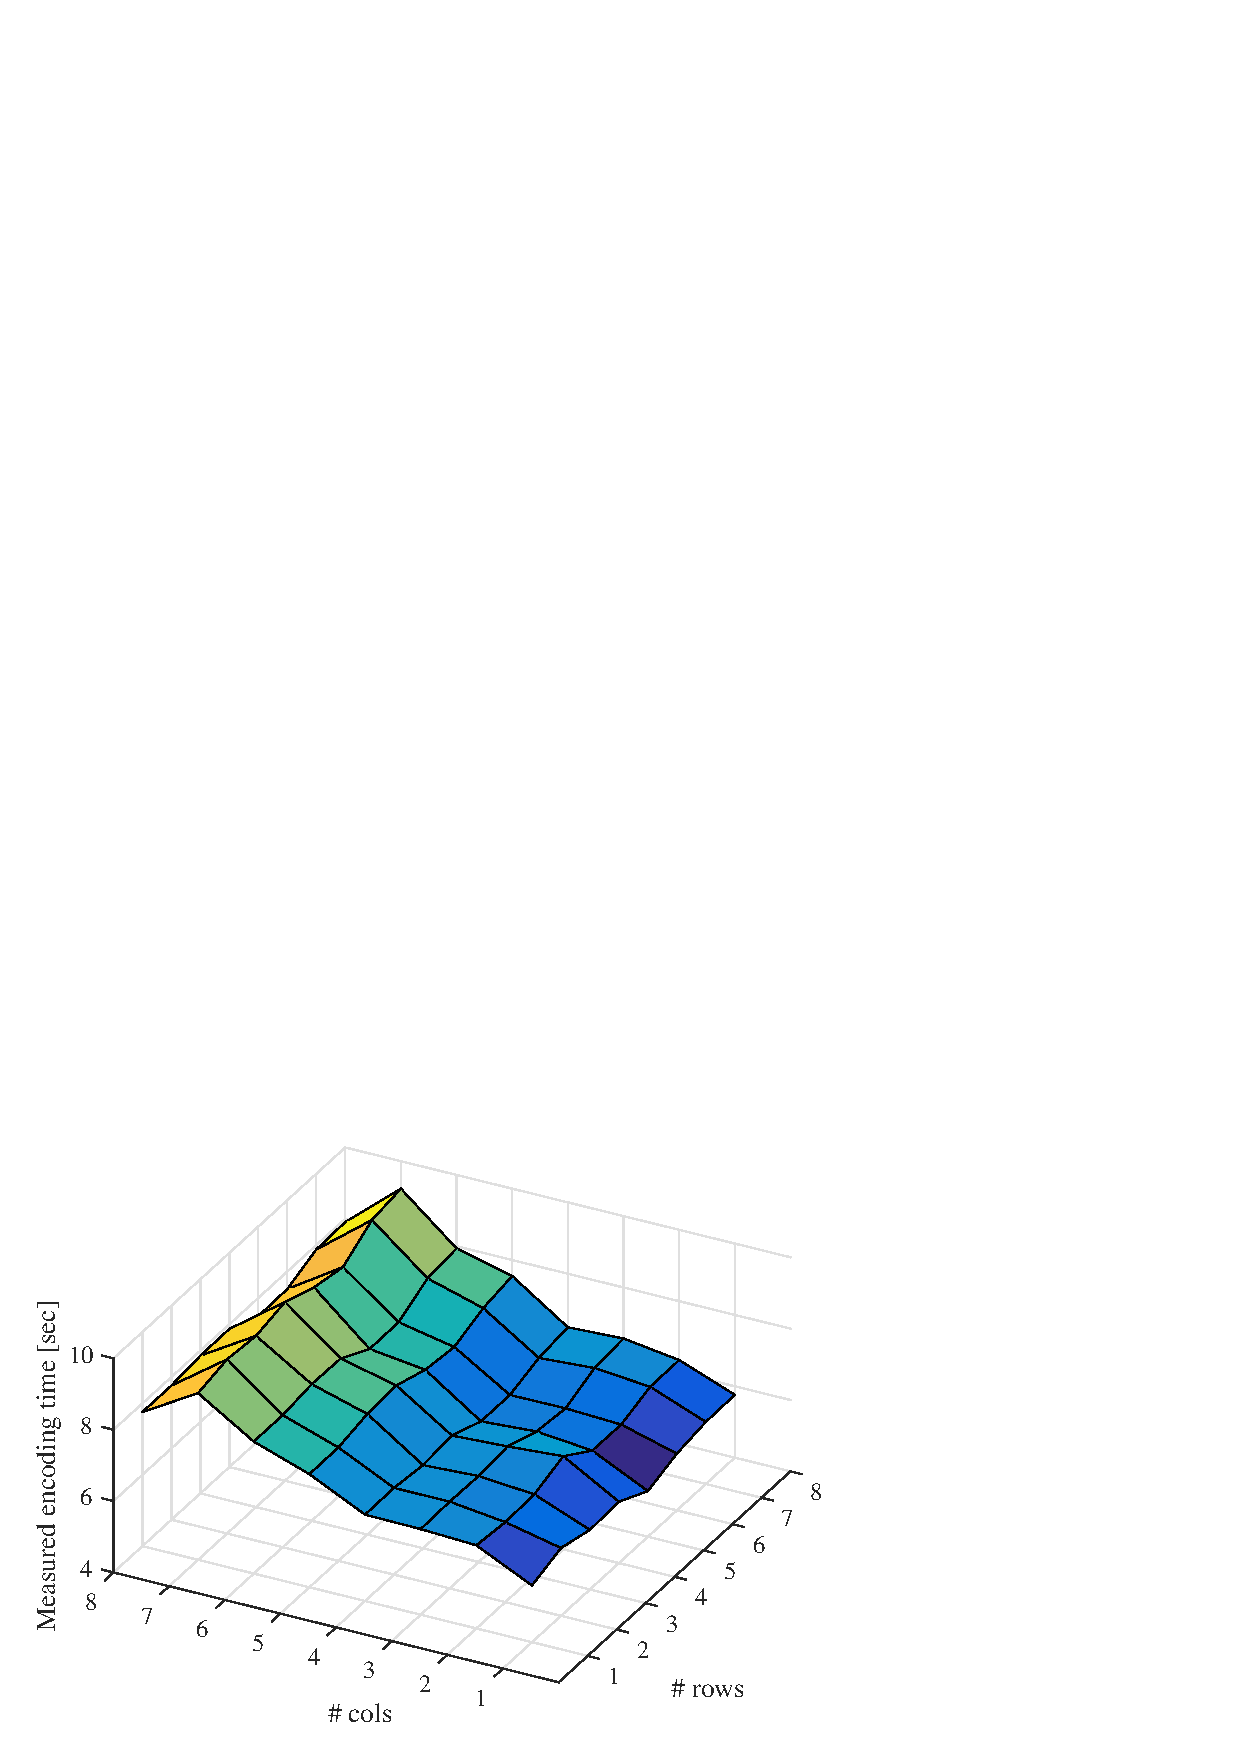
\includegraphics[width=\columnwidth]{figures/times_v1.pdf}
	\caption{Encoding time for a 30s video across tile configurations. The tile qualities alternate between high and low in a checkerboard pattern. For each configuration that has an odd number of tiles, we set the extra tile to be low quality. Note the lower encoding time for 8 columns vs 7 columns which is due to better alignment.}
	\label{fig:time}
\end{figure}

\subsection{Installing and Using RATS}

TODO: include more details if we have room

RATS was developed and evaluated on Ubuntu 18.04, using CUDA 9.2, FFmpeg 3.4, and Boost 1.64. We use a modified version of FFmpeg which sets \texttt{sliceModeData=3} and adds a new field, \texttt{numSlices}, to \texttt{AVCodecContext} in order to specify the tile configuration at run-time. FFmpeg must be configured to use CUDA and produce static libraries during compilation.

Details on the installation and usage of RATS, as well as an overview of the source code, can be found in the git repository \footnote{https://github.com/ballardt/nvenc-live}.

\section{RATS in an infrastructure}

The main contribution of RATS to the state-of-the-art is the efficient and accessible
tiling of videos with HD quality and better on a single computer equipped with a
suitable generally programmable consumer-grade GPU.
We circumvent certain limitations of the GPU and are thereby able to generate videos
that are compliant with the advanced tiling scheme of HEVC.

In the demo, we present
a variation of our solution that stitches videos comprised of tiles of various
qualities before delivery to an end-system.
This is not the only possible approach, and it is actually somewhat more complex
than the creation of distinct video streams for each individual tile.
DASH provides the extension DASH-SRD (spatial relationship description), which
allows a client to access tile stream individually, synchronize them and make
independent quality choices for each of them. Providing the appropriate data and
metadata for this approach is actually a simplification to the approach that we
demonstrate in this paper.

The remaining infrastructure for delivering the encoded video is entirely comprised
of open-source software where we make use of HTTP adaptive streaming.
The packages that have been used include NGinx\footnote{https://github.com/nginx/nginx.git}, Kaltura nginx-vod-module\footnote{https://github.com/kaltura/nginx-vod-module.git} and MediaElement.js\footnote{https://www.mediaelementjs.com/}.

%\begin{itemize}
%\item NGinx: available from \url{https://github.com/nginx/nginx.git}
%\item Kaltura nginx-vod-module: available from \url{https://github.com/kaltura/nginx-vod-module.git}
%\item MediaElement.js: available from \url{https://www.mediaelementjs.com/}
%\end{itemize}


\section{Evaluation}
To evaluate RATS, we analyze its performance across multiple tile configurations. In particular, we examine the encoding speed, output file size, and the quality of the final image. Evaluations were performed with an NVIDIA GTX 1080 Ti GPU on Ubuntu 16.04. The source video used was 30 seconds long with a resolution of $3940\times2048$ pixels. The source video was originally encoded with Apple PRORES, and FFMpeg was used to convert it to a series of raw YUV images.

Examining Figs. \ref{fig:time} and \ref{fig:size}, we see that the number of tile columns is the primary factor affecting encoder performance. Intuitively, this makes sense; the number of columns dictates the number of sub-images necessary, each of which requires two more NVENC encodes per frame and multiple stitching operations. Furthermore, stacking each tile column requires additional transformations of the source image. In contrast, tile rows are simply required to divide evenly along CTU borders, incurring minor computation costs only when they are misaligned and the source image must be cropped.

In Fig. \ref{fig:time}, there are several notable jumps which highlight various components of the RATS pipeline. The first of these occurs between 1 and 2 tile columns as the source image starts transforming and the stitcher begins to make more significant bitstream modifications. When there is only one tile column, tiles are simply rows across the whole image, and the stitching process consists mostly of picking the quality for each row without rearranging any tiles. Another such jump occurs between 4 and 5 tile columns as sub-images are introduced. Interestingly, the spike at the 7 column originates entirely within NVENC. This is likely due to the fact that the CTU width of the uncropped source image is not divisible by 7, but all other values tested are. TODO: better explanation

TODO: discuss fig. \ref{fig:size}
TODO: do other jumps originate entirely in NVENC?

%\begin{figure}[t]
%	% \includegraphics[width=\columnwidth]{figures/hevc_eval_qual.png}
%	\caption{Encoding speed vs. tile quality for $4\times4$ tiles. All tiles on the left are of the high bitrate, while those on the right are of the low bitrate.}
%\end{figure}





\begin{figure}[t]
	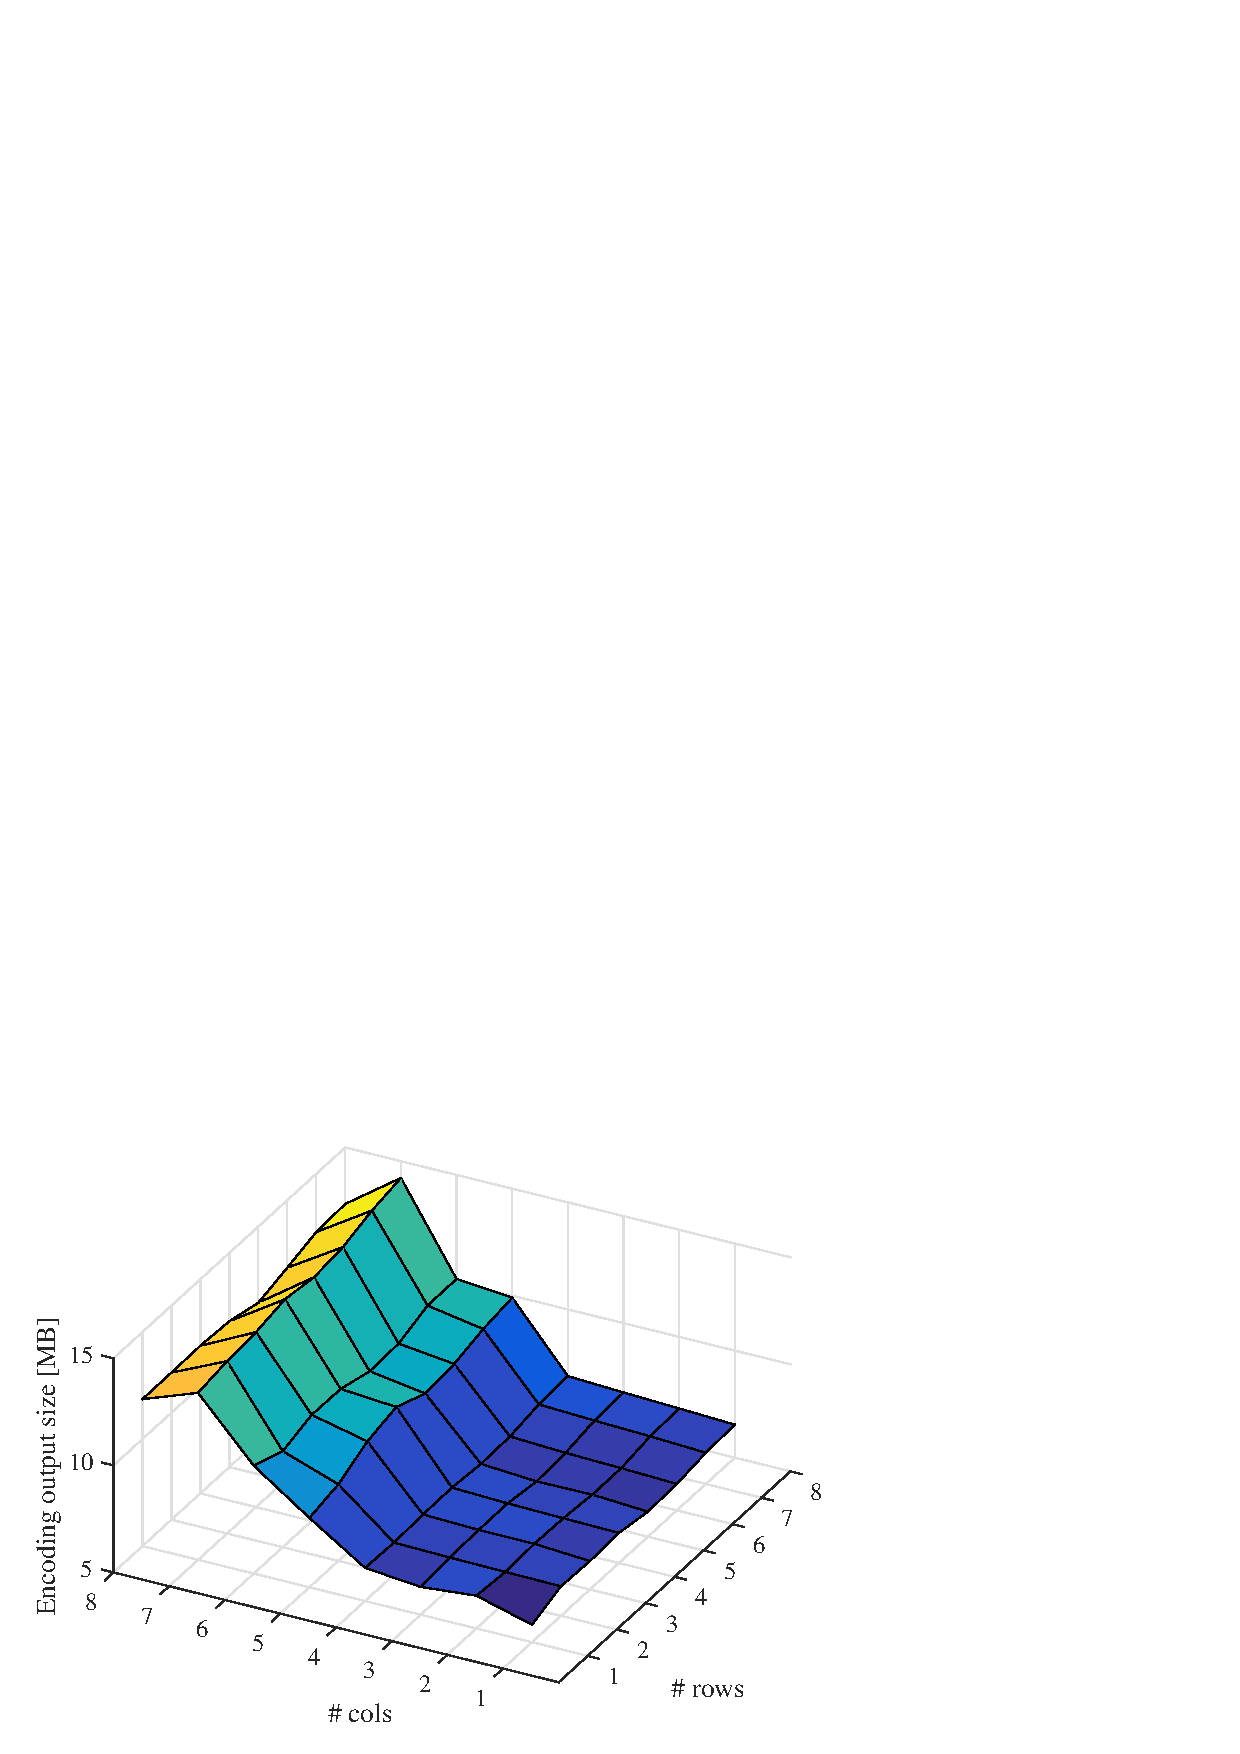
\includegraphics[width=\columnwidth]{figures/sizes_v1.pdf}
	\caption{Encoding output size in MB for a 30s video across tile configurations. The tile qualities alternate between high and low in a checkerboard pattern. }
	\label{fig:size}
\end{figure}



\section{Future Work}

TODO: Merge with section 4, then remove future work

In this work, we have focused on the problem of encoding small independent regions of a video at multiple bitrates in real-time, as this is the primary technical challenge involved in 360-degree or 4K ABR livestreaming. However, in the interest of developing a fully-realized demonstration, we intend to place this work within a web-based streaming platform where clients could watch a live video from, e.g., the web browser on their phone. There exist an abundance of tools to set up a DASH-like streaming platform for H.264, but our options are more limited with HEVC.

One potential implementation may be as follows: For each frame, the stitching process is performed multiple times with different bitrate configurations requiring different network capabilities. For example, one configuration may contain only a few high-quality tiles in very important regions, while another may use high-quality tiles almost everywhere. Important regions may be found automatically via [CITE]. These frames are placed in short video segments such that the first frame is always an I-frame. Kaltura, an open source video-on-demand platform, is used to manage these segments, and clients can stream them via MediaElementJS. This solution is analogous to DASH, using the server to store a few pre-rendered qualities in short chunks which can be requested by the client.

It may be desirable to allow the client to choose their bitrate at the tile level. For example, if a user looks in a particular direction, we may wish to increase the quality only in that area. However, this would require either that the server perform custom stitching for each client, or that the stitching component occurs in the browser on the client side. In the first case, the server would quickly be overloaded; in the second, stitching would take much longer than real-time. A better alternative may be to group users into categories based on where they are looking and produce video segments for each category. All users will be watching the stream at the same time and are likely to follow the most interesting parts of the image, so this may naturally produce videos in which important features are of a high quality. We intend to explore several of these options in a future work.

\section{Conclusion}

TODO

\section{Notes, to be deleted}
Sharing CUDA contexts (not used): https://devtalk.nvidia.com/default/topic/1031189/video-codec-sdk/sharing-the-same-cuda-context-for-encoding-nvenc-and-decoding-nvdec-/

NVIDIA patch (used): https://github.com/keylase/nvidia-patch

\begin{figure}[t]
	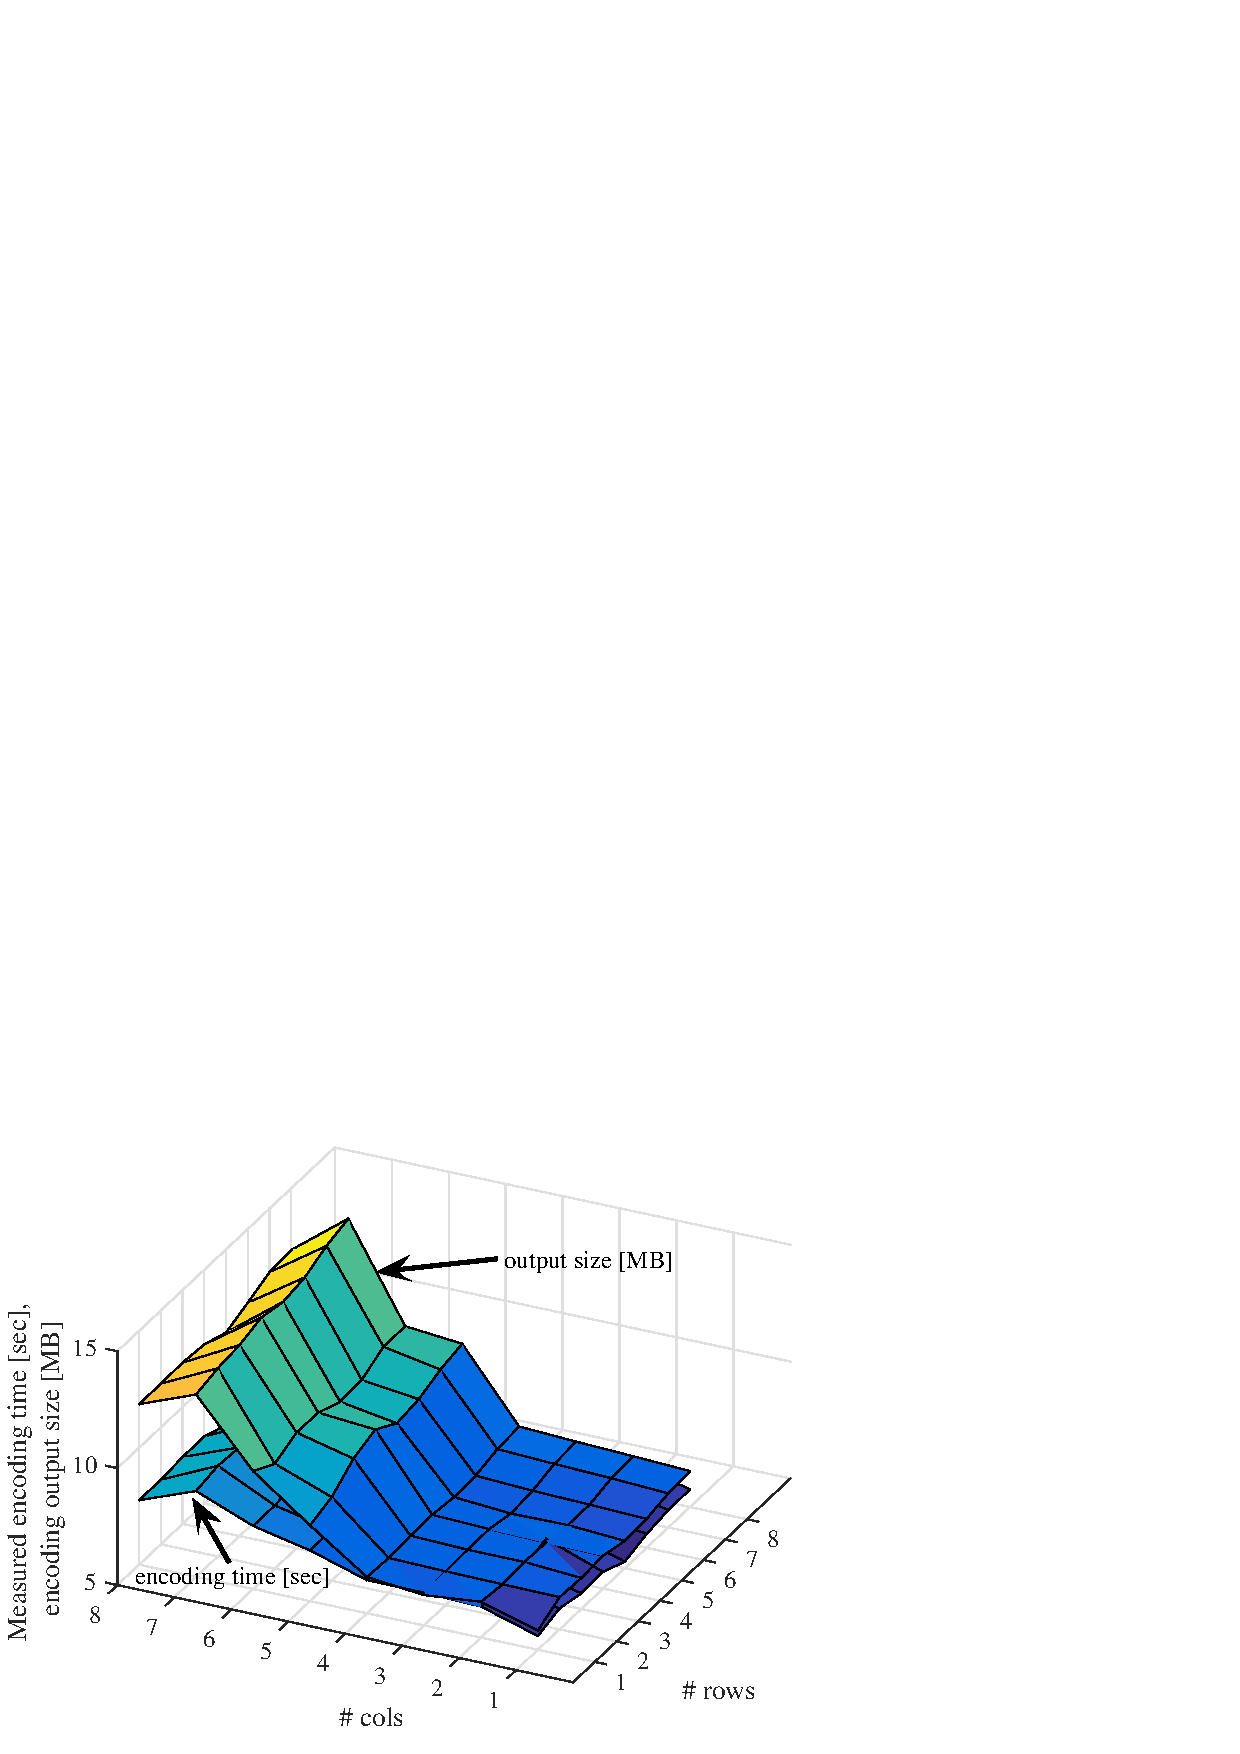
\includegraphics[width=\columnwidth]{figures/times_size_combined_v1.pdf}
	\caption{JUST FOR US. A combined view of the encoding time and the resulting output size.}
\end{figure}
